
\documentclass[conference]{IEEEtran}
\usepackage[utf8]{inputenc}
\usepackage[T1]{fontenc}
\usepackage[UKenglish]{babel}
\usepackage{cite}
\usepackage{graphicx}
\usepackage{subfig}
\usepackage{todonotes}
\usepackage[cmex10]{amsmath}
\usepackage{hyperref}
%\parskip 2ex % TODO Remove
\usepackage{dblfloatfix}
\usepackage{xfrac}

\hypersetup{
  pdftitle    = {Energy-efficient Routing Protocols for Mobile ad-hoc Networks},
  pdfauthor   = {Julian Andres Klode},
  pdfcreator  = {pdflatex on Debian GNU/Linux},
  pdfproducer = {LaTeX on Debian GNU/Linux}
}

\begin{document}
\title{Energy-efficient Routing Protocols for Mobile Ad-hoc Networks}
\author{\IEEEauthorblockN{Julian Andres Klode}
\IEEEauthorblockA{Philips-Universität Marburg \\
Email:\href{mailto:klode@mathematik.uni-marburg.de}{klode@mathematik.uni-marburg.de}}}

\maketitle



\begin{abstract}
Mobile Ad-Hoc networks, with battery-powered nodes, require energy efficient
routing protocols in order to reduce the power consumption of nodes.

Over the years, several categories of routing protocols have emerged.
This term paper gives an overview of the different categories of energy
efficient routing protocols, and samples for each category.
\end{abstract}
\begin{figure*}
  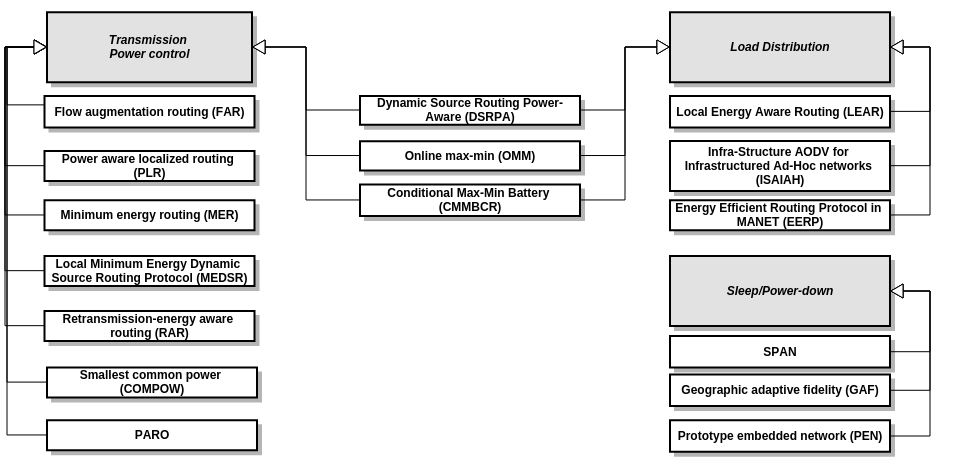
\includegraphics[width=0.9\textwidth]{images/overview}
  \caption{Overview of the protocols}
  \label{fig:overview}
\end{figure*}

\section{Introduction}
Mobile ad-hoc networks present a number of unique challenges for routing protocols.
Their nodes are battery-powered and non-stationary, requiring flexible network architecture.
One example for ad-hoc networks, albeit not particularly mobile, are wireless sensor networks.

Routing protocols in such networks need to consider several important key
factors:
\begin{enumerate}
   \item Scalability -- A protocol should scale to a large number of nodes
   \item Fault tolerance -- A protocol should continue working if some nodes fail
   \item Energy efficiency -- A protocol should not consume more energy than needed,
   either on an individual node, or aggregated.
\end{enumerate}

A recent survey\cite{alotaibi2012survey} on routing protocols for wireless
ad hoc networks describes six categories of routing protocols for wireless
ad-hoc networks,  in addition to the classic categories of proactive (that is, table driven)
and reactive (that is, on demand) routing protocols:
\begin{enumerate}
  \item Geographical
  \item Geo-cast
  \item Multi-Path
  \item Hierarchical
  \item Power-aware
  \item Flow-Oriented
  \item Hybrid
  \item WMN
  \item Multicast
\end{enumerate}

Most of these categories are not focused on energy efficiency, but more on
other factors such as fault tolerance, scalability and performance. The only
category in which energy efficiency is discussed is that of power-aware algorithms.


\section{Categories of ad-hoc routing protocols}
Classic routing protocols are categorised in two dimensions:
centralised/distributable and proactive/reactive.
The unique challenges inherent in wireless ad-hoc networks led to a larger
amount of categories, which are not always necessarily disjoint, meaning
that an algorithm may belong to one or more categories.

\subsection{Basics: Proactive and reactive routing}
Proactive and reactive routing algorithms are the basic dimensions of routing
categories.

\subsubsection*{Proactive routing}
In proactive routing algorithms, each router builds its routing table by
(regularly) exchanging messages with other routers in the network.

This has the advantage that routing information is already available when a
package is to be routed.
A huge disadvantage of proactive routing protocols is the overhead imposed
by the exchange of the update messages.

\subsubsection*{Reactive routing}
In a reactive routing algorithm, routes are discovered when a packet arrives
from a source and needs to be delivered to some destination.
While the routes need to be discovered more often than in proactive algorithms,
there is no traffic overhead due to the lack of special control messages, and
as such, the reactive approach is considered to scale better.

Two examples of reactive routing protocols are dynamic source routing (DSR)
and ad-hoc on-demand distance vector routing (AODV). The difference between
the two is that DSR, as a source routing protocol, records the entire route
in the package during the route discovery phase; and does not store routing
tables in the intermediate nodes, thus simplifying their design.

\subsection{Other categories}
Distinguishing between proactive and reactive routing algorithms gives a very
coarse categorisation. As such, several other categories have been identified
over the years.

\subsubsection*{Geographical routing}
The basic idea behind geographical routing is that nodes are addressed by
their geographic location instead of an IP address. This has the advantage
that each node does not need to know the full network topology, but each
node needs to know its location and each source needs to know the location
of the receiver.

In section~\ref{gaf} we will take a look at the Geographic adaptive fidelity (GAF)
protocol, which utilises geographical features for routing, although with an
interesting twist.

\subsubsection*{Geo-cast}
Geo-cast routing merges multi-cast routing with geographical routing, to
deliver messages to a group of nodes identified by their locations.

\subsubsection*{Hierarchical}
A hierarchical routing algorithm defines multiple zones or clusters with
gateways that connect them with each other. Inside a cluster, there often
are one or more cluster heads, that are responsible for maintaining the
connectivity within the cluster. Non-head nodes can only communicate with
their cluster heads, whereas gateway nodes can exchange information with
other clusters.


\subsubsection*{Multi-path}
In a multi-path routing algorithms, multiple paths exists from one source
to a destination. The obvious advantages of a multi-path routing
algorithm include fault tolerance (if one path fails, another is still in
use), load distribution (congested routes can be avoided by chosing alternative
routes), peak performance (multiple routes may be used in parallel for different
parts of data).

Energy-efficiency is not a paramount concern of most multi-path routing, the
load balancing idea can however not only be applied to performance, but also
to power levels, to distribute the power used within the network, as we will
see later on. Such an algorithm would of course also be power-aware.

\subsubsection*{Power-aware}
A power-aware routing algorithm tries to find a good trade off between
power consumption of nodes and mobility. Yu, Lee, Youn~\cite{main1} describe two categories
of power-aware protocols:

First, there are those algorims that try to minimise the \textit{active communication energy}. Two
subcategories can be identified:
\begin{itemize}
    \item Transmission power control -- controlling the power that is used for transmitting a packet
    \item Load control/balancing -- algorithms that distribute the load over available nodes
\end{itemize}
There also exist hybrids of the two, for example, DSRPA (section~\ref{dsrpa})
selects nodes with the freshest batteries and also controls the transmission
power.

Other algorithms do not try to minimise the active communication energy, but
instead focus on minimising the  \textit{inactivity (idle) power consumption}. For example, unused
nodes can be put to sleep or into lower power states. This subcategory often
distinguishes between master and slave nodes -- for example, SPAN (section~\ref{span}), but there are also protocols
where no such distinction is made -- for example, PEN (section~\ref{pen}).

\subsubsection*{Hybrid}
A hybrid protocol starts off as a proactive routing protocol but switches
to reactive routing for newly added nodes in order to reduce the control
overhead of proactive routing. In ad-hoc networks, it is implemented in
hierarchical network architectures.

\subsubsection*{Flow-oriented}
Alotaibi and Mukherjee~\cite{alotaibi2012survey} list flow-oriented or flow-aware
routing as another category.
Examples they list include
IERP, which most likely refers to the The Interzone Routing Protocol for Ad Hoc Networks, an Internet Draft\cite{manet-zone-ierp-02};
and SrcRR\cite{aguayo2005srcrr}, a wireless mesh network routing protocol. It is unclear what exactly
makes these routing protocols flow-aware, and in absence of any definition of
that term, it does not warrant any further discussion. 

\subsubsection*{WMN}
WMN routing algorithms are routing algorithms for wireless mesh networks.
A wireless mesh network is a special type of (ad-hoc) networks in which all
nodes participate in the distribution of data.

Over the years, multiple routing algorithms for wireless mesh networks have
been designed, examples include B.A.T.M.A.N. and the newer B.A.T.M.A.N. advanced
which is used in the Freifunk community, for example\cite{batman-adv}.
% OUT OF PLACE
\begin{figure*}
\centering
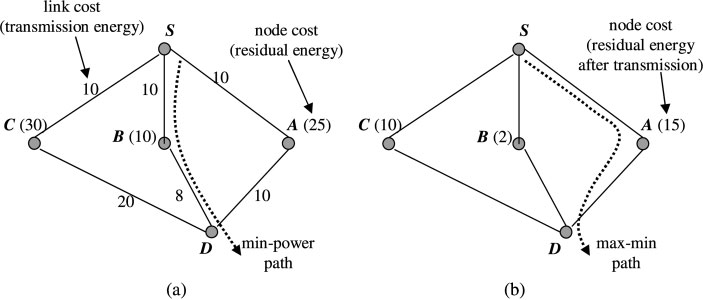
\includegraphics[width=0.7\textwidth]{images/omm}
\caption{Paths in OMM\cite{alotaibi2012survey}}
\label{ommex}
\end{figure*}
\subsubsection*{Multicast}
Multicast routing algorithms are simply routing algorithms for multicast
groups.
One example for a multicast routing algorithm is multicast ad-hoc on-demand
distance vector (MAODV)\cite{manet-maodv-00}, which is currently a work
in progress internet-draft.

\begin{figure*}
\centering
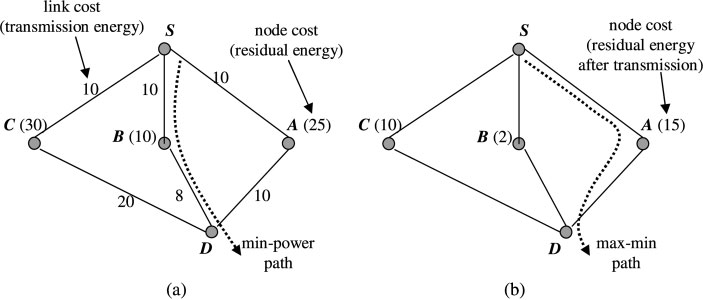
\includegraphics[width=0.7\textwidth]{images/omm}
\caption{Paths in OMM\cite{alotaibi2012survey}}
\label{ommex}
\end{figure*}
\section{Survey of energy-efficient protocols}
In the following, various routing protocols from each category (power control,
load distribution, hybrids of them, and sleep/power-down) of energy
efficient routing protocols are presented. An overview diagram can be found
in Figure~\ref{fig:overview}.
\subsection{Transmission power control}
Protocols in this category try to minimise the power required to transmit
a message. This class of algorithm is akin to a graph optimisation problem,
with the nodes in the MANET represented as nodes in a graph, the power required for
transmitting over a link $p_{ij}$ represented as the cost of a vertex, and the goal
to search the minimum-cost path between two nodes.

\subsubsection{Flow augmentation routing (FAR)}
Flow augmentation routing (FAR)\cite{chang2000energy} finds the routing
path in a (static) network that minimises the sum of link costs in the network,
where the link cost between $i$ and $j$ is defined as \( e_{ij}^{x_{i}}E_{i}^{x_{2}}R_{i}^{-x_{3}}\);
\(e_{ij}\) is the energy cost for the transmission, $E_{i}$ is the initial energy
of the node $i$ and $R_{i}$ is the residue energy of the node. \(x_{1}, x_{2}, x_{3}\)
are weighting factors. As an example, if $x_{1}=x_{2}=x_{3}=0$, then the cost
of each link is 1, and the optimal path is the shortest distance path.

In a static wireless network, $E_{i}$ and $e_{ij}$ are constant, but $R_{i}$
continues to decrease. Thus, the optimal link at one point in time might not be the
optimal link at a different point in time. FAR solves this problem iteratively:
Calculating the optimal path at each step, after updating the residual energy
and link costs.

\subsubsection{Online max-min (OMM)}
\begin{figure*}
\centering
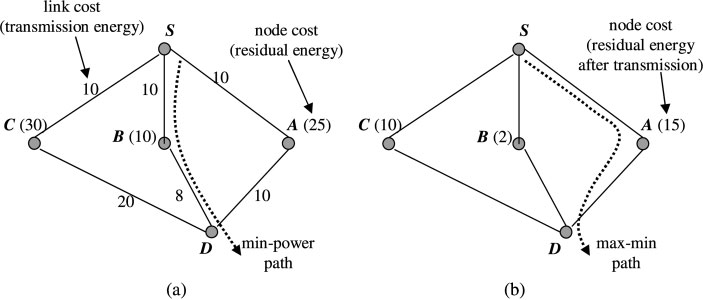
\includegraphics[width=0.7\textwidth]{images/omm}
\caption{Paths in OMM\cite{alotaibi2012survey}}
\label{ommex}
\end{figure*}
\label{omm}
OMM \cite{li2001online} maximises the network lifetime using two metrics:
\begin{enumerate}
  \item \textbf{min-power} - Minimising the overall power
  \item \textbf{max-min} - Maximising the minimum residual power
\end{enumerate}

First OMM calculates the \textit{min-power} path using Dijkstra’s algorithm. Let
the power required by that be $P_{min}$.
Then it determines the \textit{max-min} paths by looking at all paths whose
power do not deviate much from the min-power path, that is, less than $zP_{\min}$
for some $z \ge 1$. It calculates the minimum residual power of all nodes
after the transmission would have taken place, and chooses the path where
that value is largest.

For example, in Figure~\ref{ommex}, we can see that the min-power path from
$S$ to $D$ is $S \to B \to D$ with a value of 18 ($S \to A \to D$ has 20,
$S \to C \to D$ has 30).
It's minimum residual energy will be $2$, as node $B$ needs
$8$ out of the $10$ power units it has.

Looking at the alternate paths, we see that $S \to C \to D$ will have a
minimum residual energy of $30-20=10$ in node $C$, and $S \to A \to D$ will
have a minimum residual energy of $25-10$ in node $A$.
Thus, the max-min path is $S \to A \to D$.

Choosing a good value for $z$ in $zP_{\min}$ is important: For $z=1$, only
the min-power path is considered; for $z \to \inf$, all paths can be
considered. The algorithm starts with a \textit{random} value for $z$, and
then measures the residual energy (\textit{lifetime}) of of the most overloaded node during some
fixed time period. Afterwards, the value of $z$ is increased by a small constant
and the lifetime is measured again. If the lifetime increases, the value of $z$
is increased, otherwise, it is decreased. Because the lifetime is measured
in two distinct time periods, it is assumed that load distribution is roughly
similar, otherwise the results might not be really useful.


\subsubsection{Energy Efficient Routing Protocol in MANET (EERP)}
EERP\cite{main2} is a variation of DSR that stores a minimum energy field
in a route request package, which is set to 100 percent at the beginning. Each
intermediate node will then override the value if its own residual energy rate
is lower than the stored one. The packet is then forwarded if the nodes residual
energy is above a certain threshold.

Once the route requests reach the destinations, the destination picks the route
with the maximum minimum hop energy, that is the \textit{max-min} path. OMM
does something similar, but EERP seems to use the power
levels before the transmission whereas OMM uses the power levels after the
transmission and can also switch to min-power paths.

\subsubsection{Power aware localized routing (PLR)}
PLR\cite{stojmenovic2001power} is a geographical routing protocol, at least
to a certain extend, that tries to minimise the overall power usage. Each node
selects the next hop based on the power required for sending to this node, and
sending from that node indirectly to the destination.

For this, it has to know the locations of the next hops and the location of
the destinations. Based on the locations and the distance between the locations,
it can then estimate the power usage.

For direct connections, this is:
\( p(d) := ad^{\alpha} + c \)
for some constants $a$ and $c$ and some $\alpha > 2$ (that is, power usage
is at least growing quadratic in relation to the distance).

For indirect communication between the next hop and the final destination,
the power usage can be calculated as:
\begin{align*}
   q(d) &:= cn + da \left(\sfrac{a(\alpha - 1)}{c}\right)^{\sfrac{(1-\alpha)}{\alpha}}, \\
      n &:= d\left(\sfrac{(a(\alpha - 1))}{c}\right)^{\sfrac{1}{\alpha}};
\end{align*}
where $n-1$ is the optimal number of intermediate nodes\cite{stojmenovic2001power}.

So, given an example like Figure~\ref{plrexample} with a source node $A$, neighbours $N_{1}$, $N_{2}$, and $N_{3}$, and a
destination $D$, $A$ should chose the next hop as the $N_{i}$ for which
$p(|AN_{i}|) + q(|N_{i}D|)$ is minimal.

\begin{figure*}
\centering
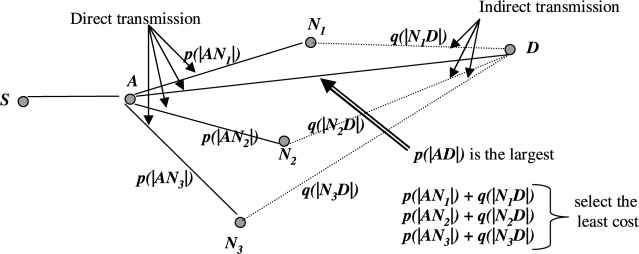
\includegraphics[width=0.7\textwidth]{images/plr-example}
\caption{Selection of next hop in PLR\cite{alotaibi2012survey}}
\label{plrexample}
\end{figure*}

\subsubsection{Minimum energy routing (MER)}
MER\cite{doshi2002demand} modifies the dynamic-source-routing (DSR)\cite{johnson1996dynamic}
and 802.11 MAC algorithms\cite{woesner1998power} with 8 options (table~\ref{tbl:mer-options}) in order to
(1) obtain power information, (2) measure overhead of energy-awareness, and
(3) maintain the minimum power route with mobile nodes.

\begin{table}[tb]
  \begin{tabular}{ll}
    Options & Implementation Level  \\
    \hline
    A: Routing packet-based power control & Routing software/\\ &802.11 firmware \\
    B: Minimum energy routing & Routing software \\
    C: Cache replies off & Routing software \\
    D: Internal cache options & Routing software \\
    E: Multi-hop route discovery & Routing software \\
    F: MAC layer ACK power control & 802.11 firmware \\
    G: Route Maintenance with power sensing & Routing software \\
    G: HMAC-Level snooping and gratious replies & 802.11 firmware \\
  \end{tabular}
  \caption{Options in MER}
  \label{tbl:mer-options}
\end{table}

Option $A$ modifies \textit{route-request} packages of the DSR protocol to
include the power used by the sender, which can the be added to the power
of the receiver to calculate the minimum power required for transmissions
from that sender to it. The value is appended at each intermediate node, and the
destination node then includes it in its \textit{route-reply} header.

The source node than includes this information when it's sending a packet, and
all nodes transmit that package with the controlled power level.

Option F does the same for the MAC layer's ACK packets.

Option $B$ is related to the route cache of the DSR protocol ($C$ and $D$ as well). It
uses the information obtained by option $A$ to select the route that requires
the minimum energy amongst its cached routes.

Option $G$ takes care of adjusting routes when the power transmittion requirements
change because nodes moved.

Option $E$ and $H$ allow nodes not participating in the routing to recommend
alternative, more energy-efficient, routes.
\subsubsection{Local Minimum Energy Dynamic Source Routing Protocol (MEDSR)}
MEDSR\cite{tanque2007minimum} modifies the messages of the DSR protocol to
provide zero-overhead (as in: no extra control messages) energy-aware routing.

MEDSR uses two power levels for route discovery: A low one, and a high one. If
the source does not receive a reply for three route request messages at low
power, it switches to the high power level.

In contrast to other algorithms like MER, it only stores one power level field
in the packets, rather than one power-level per link. That power level is stored
in amended route request and route reply packets.

When a node $C$ receives a route reply from a node $D$, it can estimate the
power level required for transmitting to $D$ by calculating:
\[ P_{min} = P_{tx} - P_{recv} + P_{th} \]
where $P_{tx}$ is the transmit power of $D$, $P_{recv}$ the receive power of $C$,
and $P_{th}$ is the threshold power for a successful receive. In 802.11, that's
usually $3.652 \cdot 10^{-10}$ watt. In order to avoid instability of the link, a margin is added
\[ P_{min} = P_{tx} - P_{recv} + P_{th} + P_{margin}\].{}

In addition to the usual tables maintained by DSR, MEDSR also stores a power
table at each node: For each node, the minimum power required to reach it.

\subsubsection{Retransmission-energy aware routing (RAR)}
Transmissions may have link errors which require re-transmitting packets over
a link. A path with many short links might be more efficient than a path with
few long distance links in the absence of link errors, but with link errors,
things might look different, because some packets need to be re-transmitted.

RAR\cite{banerjee2002minimum} modifies the cost/power requirement of a link $p_{i,i+1}$ by including the error rate of that
link $e_{i,i+1}$. That modified link cost $P_{i,i+1}$ is defined as
\[ P_{i,i+1} = \underbrace{p_{i,i+1}}_{\text{original link cost}} \cdot \underbrace{\sfrac{1}{\overbrace{(1-e_{i,i+1})}^{\text{success rate}}}}_{\text{expected number of tries}}. \]

\subsubsection{Smallest common power (COMPOW)}
Network protocols often require handshaking of some sorts, like acknowledgements
sent to a sender for his packages. Thus, for a MANET to be reliable for those
protocols, for every two nodes, there must be routes in both directions, that
is, some form of bi-directionality.

The smallest common power\cite{narayanaswamy2002power} achieves bi-directionality
of communication in the network.
It does so by maintaining a smallest common transmission power for all nodes,
chosen so that all nodes can communicate with each other. If the power is too
low, some nodes could not reach some others, if it is too high, there might be
many redundant paths. See Figure~\ref{compow:power-choice}.


\begin{figure*}
\centering
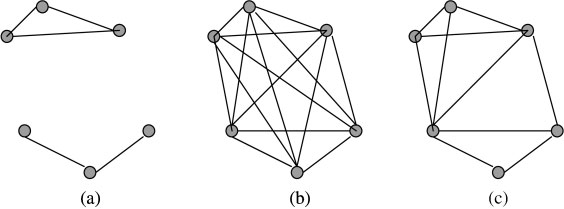
\includegraphics[width=0.7\textwidth]{images/compow-level-choice}
\caption{Power choice in COMPOW: (a) too low, (b) too high, (c) optimal}
\label{compow:power-choice}
\end{figure*}

COMPOW assumes a discrete set of power levels $P_{i}$ and maintains routing
tables ${RT}_{P_{i}}$ containing all nodes reachable from the current one. The
optimal power level $P_{i}$ can be determined as the smallest one for which
$\mid RT_{P_{i}} \mid$ is equal to the number of nodes in the network, by
exchanging the routing tables between nodes.

\subsubsection{PARO}
The PARO Protocol\cite{gomez2003paro} introduces intermediate nodes into a
route, increasing the length of the route, in order to reduce the transmission
power required by each node.

\subsection{Load distribution}\label{load-distribution}
Power-aware load distribution (or `control') algorithms distribute the
traffic based on the energy levels of the routers.
They do not try as much as the other algorithms to minimise the power required,
but instead focus more on distributing the power requirements among the available (routing) nodes.

\subsubsection{Local Energy Aware Routing Protocol (LEAR)}
LEAR\cite{woo2001non} is a variant of DSR.
Its main behavioural change lies in the forwarding of \textit{route-request} messages.
In LEAR, nodes only forward \textit{route-request} messages if their residual
energy level is above a certain threshold. Otherwise, the message is dropped
and the node does not take part in forwarding packages.

The threshold value is defined locally and changes with the time, decreasing
as the battery level decreases. If a source does not get a reply to its
route-request message, it will resend it. Nodes receiving the message multiple
times then lower their threshold value to allow the forwarding to continue.

DSR also employs a route cache. Obviously, just returning an existing node
from the route cache would not take energy level changes into consideration.
Thus, when a route is found in the cache, a new message called \textit{route-cache}
is sent via unicast to the next hop, which then forwards it to the end. This
produces far less traffic than the \textit{route-request} messages, which are
sent using broadcast messages.

\subsubsection{Infra-Structure AODV for Infrastructured Ad-Hoc networks (ISAIAH)}
ISAIAH\cite{lindgren2002infrastructured} is an ad-hoc distance vector routing
algorithm. It routes similar to AODV, but selects routes that pass through
so called power base station (PBS) instead of mobile nodes, in order to reduce
the power consumption of the mobile nodes.

As with PARO, the routes chosen by this algorithm are longer than strictly necessary, but
because more nodes are stationary, the power consumption on the mobile nodes
is reduced.

\subsubsection{Energy Efficient Routing Protocol in MANET (EERP)}
EERP\cite{main2} is a variation of DSR that stores a minimum energy field
in a route request package, which is set to 100 percent at the beginning. Each
intermediate node will then override the value if its own residual energy rate
is lower than the stored one. The packet is then forwarded if the nodes residual
energy is above a certain threshold.

Once the route requests reach the destinations, the destination picks the route
with the maximum minimum hop energy, that is the \textit{max-min} path.
OMM\cite{li2001online} does something similar (see section~\ref{omm}), but EERP seems to use the power
levels before the transmission whereas OMM uses the power levels after the
transmission and can also switch to min-power paths.

\begin{figure*}
\centering
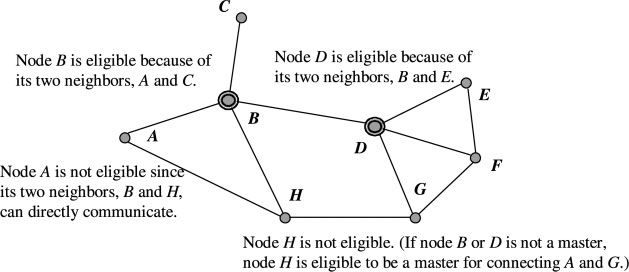
\includegraphics[width=0.8\textwidth]{images/span-master-example}
\caption{Master eligibility rule in the SPAN protocol\cite{alotaibi2012survey}}
\label{spanmaster}
\end{figure*}
\subsection{Combining Power control and Load balancing}

\subsubsection{Dynamic Source Routing Power-Aware (DSRPA)}
\label{dsrpa}
Dynamic Source Routing Power-Aware (DSRPA)\cite{djenouri2006new} defines a
power-aware variation of dynamic source routing.
 It trades of battery freshness and power consumption by defining a
metric on which it bases its routing.

Power consumption is reduced by recording the transmission power in route
request messages and then using that value and the reception power to calculate
the required power at the receiver side.

Nodes can share their power state by broadcasting in its neighbourhood a special
$E_{state}$ packet that contains the current power value. This packet is send
each time a certain percentage of power has been consumed. For example, if the
rate is set to $25\%$, a packet will be sent after 25, 50, and 75 per cent of
power consumed.

The metric representing the optimality of a a route $C=I_{0}, \ldots, I_{n-1}$
is defined as the minimum of $Opt_{c}$ (\ref{eq:dsrpa:opt-c}), where
\begin{itemize}
    \item $\alpha$ is a weight
    \item $eng(I_{i}) \in [0,1]$ is the rate of energy consumed by $I_{i}$,
    \item $Pow(I_{i}, I_{i+1})$ is the power required for the link from $I_{i}$ to $I_{i+1}$, and
    \item $MaxPow(I_{i})$ is the maximum power of the node $I_{i}$, that is, the power that allows
          it to cover its power range.
\end{itemize}

\begin{align}
Opt_{c} &:= \sum_{i=0}^{n-2} \frac{\alpha}{\underbrace{1-eng(I_{i})}_{\text{residual energy rate}}} + \frac{1-\alpha}{\underbrace{1-\frac{Pow(I_{i}, I_{i+1})}{MaxPow(I_{i})}}_{= 1 - \text{rate of total power}}}
\label{eq:dsrpa:opt-c}
\end{align} 


The more $\alpha$ increases, the more nodes with fresh batteries are preferred
(and the more $\alpha$ decreases, the more min-power routes are preferred).

We can define $\alpha$ as a function of time (\ref{eq:dsrpa:alpha}),
where $EngDiff \in [0,1]$ is the difference between the maximum and minimum rate
of energy consumed in the network and $\alpha_{0}$ some initial value.
\begin{align}
    \alpha &:= \sqrt{(1-\alpha_{0})^{2} \cdot EngDiff + \alpha_{0}}
    \label{eq:dsrpa:alpha}
\end{align}

This counters the increasing difference $EngDiff$ because if that
difference increases, $\alpha$ increases, and thus fresher nodes are preferred,
and therefore, the value of $EngDiff$ decreases.

DSRPA disperses data over multiple routes.  While normal DSR only uses one
`optimal' route, DSRPA can discover and use multiple nodes if the route request
packet contains a \texttt{ALLROUTES} flag.

It will then use non-optimal routes to distribute the load of the network like
this:

If $\#packets$ is the number of packets to be sent and
$\#paths$ is the number of paths from the source to the
destination, and the routes are ordered according to their optimality,
with 0 being the best, then the number of packets to be sent on the route $i$
is given by (\ref{eq:dsrpa:packets}).
\begin{align}
     \#packets_{i} &:= \left\lceil \frac{2^{\# paths - i - 1} \cdot \# packets}{2^{\#paths} - 1} \right\rceil
     \label{eq:dsrpa:packets}
\end{align}

This ensures that most packets are delivered on the optimal route $i=0$, and
the package count in a less optimal route is less than the count in a more
optimal route. The number of packets send on a route $i$ is approximately
twice as much as the number of packets send on the route $i+1$.

The data dispersal requires more energy than would be needed without it. It
does however minimise the difference in energy states. The decision of whether
to use data dispersal or not must be made on a per-network basis: Networks
enjoying high connectivity will consume more power with data dispersal than
networks with low connectivity, because there will be a lot more broadcasting.

\subsection{Sleep/power­ down mode}
Algorithms in this category try to minimise the time a node is active, and
maximise the time a node is at sleep. A common apprach to do this is to select
one or more masters from a set of nodes which take over the routing functionality
while the others can safely sleep. In such a scheme, nodes periodically wake up
and elect a new master if the current one goes away.

We will take a look at two master slaves protocols: SPAN, GAF;
and at one protocol called PEN that has no concept of master and slave nodes.

\subsubsection{SPAN}\label{span}
%SPAN-FIGURE
In Span\cite{chen2002span}, a master is selected based on the following rule:
A node becomes a master if two of its neighbors cannot reach each other directly
or via one or two masters. For example, in Figure~\ref{spanmaster}, nodes B and
D become masters.

In order to prevent or reduce overloading of masters, masters periodically
check whether they should withdraw from being master; and non-master nodes
periodically check if they should become master.


\subsubsection{Geographic adaptive fidelity (GAF)}
\label{gaf}
\begin{figure*}[!t]
\subfloat[Grid example]{%
  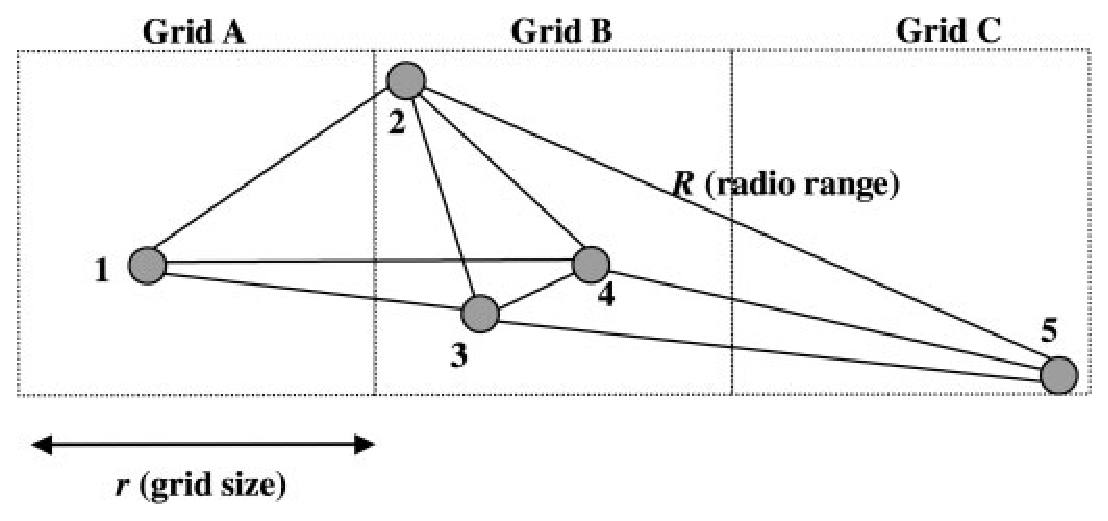
\includegraphics[width=0.46\textwidth]{images/gaf-grids}
  \label{gafgrids}
}
\hfill
\subfloat[Node states]{%
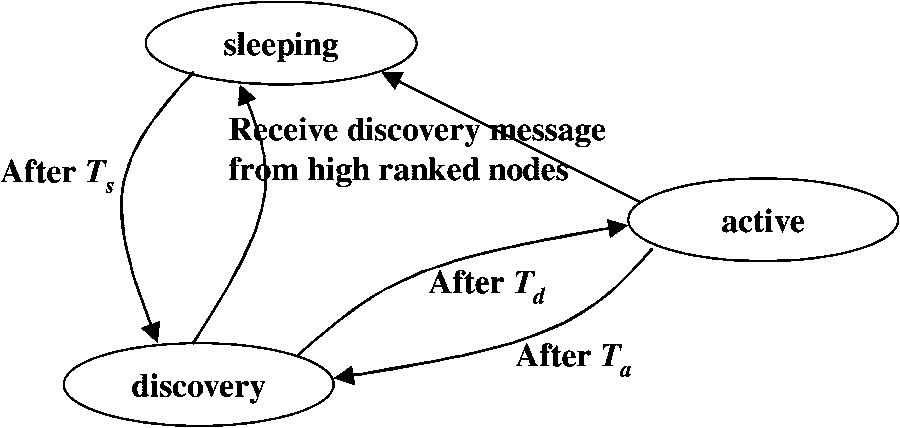
\includegraphics[width=0.46\textwidth]{images/gaf-states}
\label{gafstates}
}
\caption{Example grid and state diagram for GAF from \cite{alotaibi2012survey}}
\end{figure*}
GAF\cite{xu2001geography} uses the geographical (GPS) location of a node in
order to position them into a virtual grid.

Within each grid, the node with the highest residual energy becomes the master
of the grid, responsible for routing messages through that grid, while the
slave nodes can be put to sleep and will alternate between sleep and listening
states. For example, in grid B of Figure~\ref{gafgrids}, one of 2,3,4 can be the
master of grid B and forward messages between A and B, while the other two can
be put to sleep.

Nodes have three states, as shown in Figure~\ref{gafstates}: active for some time span $T_{a}$, in which they
act as the master of the grid; discovery for some time span $T_{d}$, in which a
master is elected - a node becomes the master if it hears no more discover messages
for time span $T_{d}$; and finally, a node can be sleeping.


\subsubsection{Prototype embedded network (PEN)}\label{pen}
PEN\cite{girling2000design} does not follow the usual master-slave scheme
used by the other protocols. Nodes periodically wake up, advertise their
presence
by broadcast messages, and then listen for any communication requests before
powering down again.

A sending node waits until it receives a broadcast message from the intended
destination, then sends a communication request to the destination during
the destinations listening period. Finally, it starts the communication.

This scheme easily avoids the cost of selecting a master and of overloaded
masters. It is only effective for networks without much traffic, as the delay
can be quite high because senders need to wait for receivers to wake up.




\section{Conclusion}
There are many different approaches to energy-efficient routing in
mobile ad-hoc networks.

Given the prevalence of protocols that minimise active communication energy,
and especially of those that rely on power control rather than load control, it
is safe to say that research has focused mostly on this category.

Section~\ref{survey} explored various ways to minimise the energy required for sending
messages, for example, PARO, which introduces closer intermediate nodes,
in order to reduce the distance between nodes, and thus their
power consumption.

Section~\ref{load-distribution} described various load distribution algorithms that distribute
the load according to the energy levels of the routers. Especially if not all
nodes in an ad-hoc network are mobile, this approach makes sense: It is
pointless to deliver messages through battery-driven routers when they can
also be forwarded by stationary nodes that are connected to a power supply.

Section~\ref{sleep} shows two basic approaches to sleep/power-down optimisation, master-slave
and the PEN protocol. Out of these, the master-slave approach seems like the
best choice for most networks, due to the almost-always available master nodes,
whereas the PEN protocol is only useful for networks without much interaction,
due to senders having to wait for destinations to be up.


\bibliographystyle{IEEEtran}
\bibliography{IEEEabrv,manets}

\end{document}


